\chapter{Discusi\'on} 
\label{ch:discusion}

A lo largo de este trabajo presentamos como parcelar la corteza cerebral
en base a un criterio estructural; estudiamos una de las m\'etodos
existentes actuales y presentamos un m\'etodo propio. En los cap\'itulos
1 y 2 introdujimos la parcelaci\'on estructural y sus fundamentos 
te\'oricos. En las secciones \ref{sec:clustering_moreno} y 
\ref{sec:analisis_moreno} analizamos el m\'etodo de parcelamiento de
Moreno-Dominguez \cite{Moreno-Dominguez2014}. El mismo
se basa en combinar un algoritmo de tractograf\'ia y otro de 
\textit{clustering} para parcelar la corteza cerebral. Luego, bas\'andonos
en su trabajo, propusimos en la secci\'on \label{ch:nuestro} un nuevo
algoritmo de \textit{clustering}. En este \'ultimo cap\'itulo vamos a discutir los resultados obtenidos. Comenzando por la robustez del
algoritmo de tractograf\'ia utilizado; siguiendo con una comparaci\'on
entre nuestro m\'etodo y el de Moreno-Dominguez; continuando con la
validez biol\'ogica de la parcelaci\'on obtenida y propondremos objetos de
futuro estudio. \\

\section{Convergencia del algoritmo de tractograf\'ia}

Nuestro m\'etodo de $clustering$ se basa en agrupar tractogramas. 
Generamos cada tractograma usando el algoritmo \ref{alg:itract} de la 
secci\'on \ref{sec:convergencia}. Los tractogramas creados de esta manera
son inherentemente estoc\'asticos. Implementamos el algoritmo 
\ref{alg:bootstrap} de la secci\'on \ref{sec:convergencia} para estudiar
si la creaci\'on de los tractogramas era estable. Esto es, si dado un 
n\'umero suficientemente grande de part\'iculas el resultado converge
a un \'unico tractograma. Las figuras \ref{fig:s1}, \ref{fig:s2} y 
\ref{fig:s3} de la secci\'on \ref{sec:resultado_estabilidad} muestran que
la desviaci\'on est\'andar es casi nula al usar $15000$ part\'iculas. A su
vez, la figura \ref{fig:mv} muestra lo r\'apido que converge la media de
tres voxels distintos. 
Como eran los de mayor desviaci\'on est\'andar, podemos asegurar que casi
no existe diferencia en la media de los tractogramas creados con $2000$
part\'iculas. El algoritmo utilizado en el trabajo demostr\'o ser estable.
\\

Nuestro m\'etodo de parcelamiento se basa en el clustering de 
tractogramas. Por ello es importante contar con un algoritmo de 
tractograf\'ia robusto. No encontramos estudios previos donde se analizara
este aspecto del algoritmo de tractograf\'ia usado. \\


\section{Comparaci\'on entra ambos m\'etodos de clustering}

En la secci\'on \ref{sec:clustering_moreno} presentamos el m\'etodo para
parcelar la corteza de Moreno-Dominguez. Luego, en la secci\'on
\label{ch:nuestro} presentamos nuestro m\'etodo. El resultado de parcelar
el \'area de Broca con estos se pueden ver en las secciones 
\ref{sec:moreno_broca} y \ref{sec:nuestro_broca}. En la secci\'on 
\label{sec:acercamiento} presentamos los resultados lado a lado en detalle
para compararlos. Los resultados son visualmente parecidos en todos los
casos. \\

Luego utilizamos ambos algoritmo para parcelar el hemisferio izquierdo del
mismo sujeto. Los resultados se encuentran en las secciones 
\ref{sec:corteza_moreno} y \ref{sec:corteza_nuestro}. En este caso 
resulta dif\'icil comparar visualmente las parcelaciones. M\'as a\'un, es
complicado encontrar cortes en los dendrogramas que generen
representaciones parecidas. Dado que los arboles fueron generados
de manera distinta, sus cortes no tienen por que corresponderse. Sin
embargo, la secci\'on \ref{sec:acercamiento_corteza} muestra algunas
similitudes en: la corteza motora y la somest\'esica; el l\'obulo frontal;
el l\'obulo occipital y el \'area de Broca. \\

Respecto a la eficiencia computacional, en la secci\'on 
\ref{sec:nuestro_clustering} comparamos ambos m\'etodos. 
Mostramos que nuestro m\'etodo permite mejorar la complejidad temporal y
espacial en al menos un orden de magnitud. Nuestro algoritmo de clustering
posee complejidad espacial $O(s^2)$ contra $O(s^2 + sm)$ del m\'etodo
Moreno-Dominguez. La complejidad temporal de nuestro algoritmo es $O(s^2m)$
contra $O(s^2)$ del m\'etodo Moreno-Dominguez. Recordemos de la secci\'on
\ref{sec:ralas} que dentro del contexto de este trabajo $m >> s$. En
general el n\'umero de semillas usadas es muy menor a la cantidad de
voxels de los tractogramas. En nuestro caso particular $s \cong 22000$ y
$m \cong 3500000$. $m$ es $159$ veces mas grande que $s$. Esto significa
que la complejidad de nuestro m\'etodo es significativamente menor a la
del m\'etodo de Moreno-Dominguez. \\


\section{Correlato con otras parcelaciones de la literatura}

Nuestro m\'etodo divide la corteza cerebral bas\'andose en un criterio
puramente estructural. Una pregunta interesante es si nuestra parcelaci\'on
posee correlaci\'on con otras anat\'omicas o funcionales. La relaci\'on
entre el aspecto anat\'omico o funcional del cerebro y su aspecto
estructural es un problema abierto en neurociencia. En particular, 
Moreno-Dominguez \cite{Moreno-Dominguez2014} hace 
una breve comparaci\'on entre sus resultados y un mapa 
citoarquitect\'onico. En nuestro caso, en las secciones 
\ref{sec:corr_anatomica} y \ref{sec:corr_funcional} comparamos nuestro 
resultado con una atlas anat\'omico basado en Desikan et al. 
\cite{Desikan2006} y un estudio funcional hecho en Bach \cite{Barch2013}.
Repetimos aqu\'i algunos de los resultados para poder discutirlos. \\

En la secci\'on \ref{sec:corr_anatomica} proyectamos 9 regiones del \'atlas
anat\'omico sobre una parcelaci\'on obtenida con nuestro m\'etodo. Esto
se puede ver en la figura \label{fig:an2pa2}. Luego
calculamos que porcentaje de las parcelaciones quedaba dentro de las
proyecciones; que porcentaje quedaba fuera y cuantas quedaban dentro de
una sola proyecci\'on. El $90\%$ del \'area de las 9 proyecciones estaba
pintada y solo un $5\%$ del \'area de nuestras parcelas quedaron fuera de
las proyecciones. A su vez, la mayor\'ia de nuestras parcelas quedaron 
dentro de una sola proyecci\'on. Nuestra parcelaci\'on cre\'o \'areas bien
delimitadas dentro de al menos 9 regiones anat\'omicas. \\

Luego repetimos el procedimiento con una parcelaci\'on obtenida con el 
m\'etodo de Moreno-Dominguez. 
En ese caso el $75\%$ del \'area de las 9 proyecciones estaban pintadas y 
un $15\%$ del \'area de las parcelas quedaban fuera de las proyecciones. 
Sin embargo esto no quiere decir que el m\'etodo de Moreno-Dominguez 
posea menor correlaci\'on con el atlas anat\'omico. La parcelaci\'on 
resultante en ambos m\'etodos depende de la altura a la cual se decida 
cortar el dendrograma. Cortando el mismo dendrograma a mayor profundidad
se pueden conseguir resultados similares a los de nuestro m\'etodo.\\

En la secci\'on \ref{sec:corr_funcional} estudiamos la superposici\'on 
entre la misma parcelaci\'on obtenida con nuestro m\'etodo y mapas de 
activaci\'on funcionales. La superposici\'on entre superficies fue 
calculada con la ecuaci\'on \ref{eq:super}. Generamos las tablas 
\ref{tb:zscore5} y \ref{tb:zscore7}. Estas muestran los valores obtenidos
para algunas regiones y mapas de activaci\'on a los cuales se les aplic\'o
un $threshold$. Dichas regiones junto con los mapas de activaci\'on se 
pueden ver en las figuras \ref{fig:32k, fig:32k_z5, fig:32k_z7}. Analicemos
una a una las regiones marcadas en de estas figuras teniendo en cuenta el 
la relaci\'on anat\'omica. La regi\'on etiquetada como $1$ es
funcionalmente consistente
con la resoluci\'on de problemas matem\'aticos. Las regiones $2-10$ son
consistentes anat\'omicamente con la corteza motora. A su vez, tambi\'en
son consistentes con el hom\'unculo cortical. El hom\'unculo cortical,
definido por Penfield \cite{Penfield1954}, es una divisi\'on funcional de
la corteza motora y de la corteza somest\'esica. Mapea distintas 
regiones del cuerpo con regiones de la corteza como puede verse en la
figura \ref{fig:homunculo}. Las regiones $11$ y $12$ son consistentes 
anat\'omica y funcionalmente con el l\'obulo temporal superior.
Finalmente, las regiones $13$ y $14$ son consistentes anat\'omica y
funcionalmente con el l\'obulo occipital. Estos resultados son prometedores
y motivan a seguir estudiando el m\'etodo propuesto.\\fig:32k

\begin{figure}[h!]
    \centering
    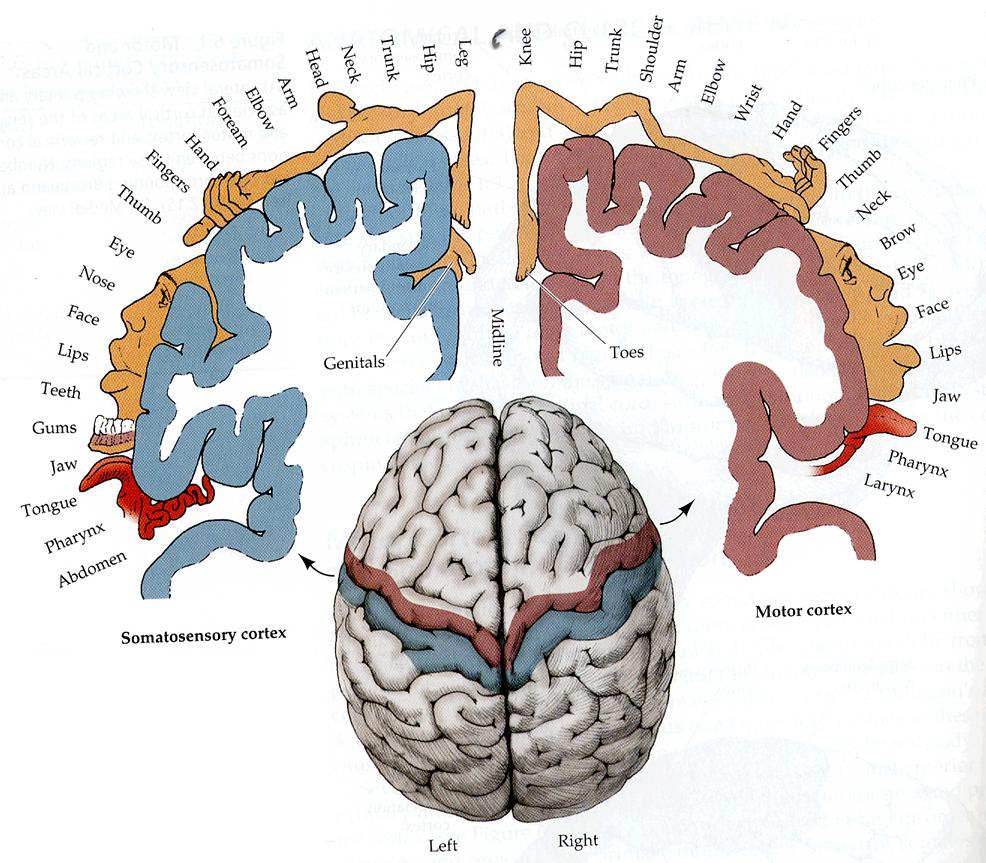
\includegraphics[width=0.8\textwidth]{img/homunculus.jpg}
    \caption{El Hom\'unculo Cortical es una divisi\'on funcional de la 
             corteza motora y la corteza somest\'esica }
    \label{fig:homunculo}
\end{figure}

\section{Trabajo Futuro}
En este trabajo presentamos un nuevo m\'etodo para parcelar la corteza
cerebral mediante el agrupamiento de tractogramas. El m\'etodo mostr\'o
resultados con una fuerte correlaci\'on anat\'omica y funcional sobre el
sujeto estudiado. Por eso es importante seguir estudiando algunos aspectos
del proceso de parcelamiento. Primero, los tractogramas aqu\'i utilizados
fueron generados con el algoritmo \ref{alg:itract} de la secci\'on 
\ref{sec:convergencia}. Ser\'ia interesante estudiar los resultados
que se obtienen al usar otros algoritmos de tractograf\'ia. Segundo, 
en las secciones \ref{sec:clustering_moreno} y \ref{sec:nuestro_clustering}
se puede ver que ambos m\'etodos de $clustering$
cuentan con un par\'ametro $k$. Este par\'ametro indica la cantidad de iteraciones a realizar uniendo solo $clusters$ vecinos y de tama\~no
similar. En el trabajo de Moreno-Dominguez \cite{Moreno-Dominguez2014} 
muestran una forma de calcular dicho par\'ametro para su m\'etodo. Hay
que estudiar una forma de calcularlo para el nuestro. Tercero, habr\'ia
que aplicar el m\'etodo sobre una poblaci\'on de sujetos y ver su
estabilidad. Esto es, estudiar si los resultados son igual de buenos que
con el sujeto aqu\'i elegido. Finalmente, en la secci\'on 
\label{sec:logit} mostramos que es posible aplicar operaciones
lineales en el espacio $LogOdds$. Esto puede utilizarse en particular para
calcular el tractograma medio de una poblaci\'on de sujetos. En estudios
futuros analizaremos el crear un atlas de la corteza basado solo en
informaci\'on estructural.\\

